\chapter{Algebraic effects and effects handlers}
\label{cpt-alg-eff}

  \section{Algebraic effects in Frank}
  \label{cpt-alg-eff:frank}

  Algebraic effects and effects handlers provide an alternative to monads and monad
  transformers way to express effectful computations. Building parser combinators in
  term of algebraic effects and the process of parsing as their handlers is a solid
  model problem to find out strengths and weaknesses of this approach.

  This section describes a prototype implementation of parser
  combinators library in experimental programming language
  Frank~\cite{DBLP:conf/popl/LindleyMM17} which has first-class support for
  algebraic effects and effects handlers. Parsers may be represented either by
  combination of multiple effects, for instance, mutable state and possible failure,
  or may be expressed as a monolith effect signature. In conclusion, we make a
  note on expressive power of Frank's implementation of algebraic effects and
  handlers.

  \subsection{Building parsers as a combination of effects}

    Section~\ref{cpt-effects:alg-effects} gives an account on algebraic effects and
    effects handlers and, in particular, on programming with these concepts in Frank
    programming language. This section employs Frank to build a prototype of parser
    combinators library.

    \subsubsection{Defining parser combinators}

    As is has been already said, simple parser could be expressed as a computation
    with two effects: state of input stream and a possibility of failure. Thus,
    handling parsing means handling a combination of those two effects, that is done
    by composing handlers for failure and state (see
    listing~\ref{listing:parserHandlerCombo}).

    \begin{figure}[h]
    \begin{lstlisting}
parse : {[Error, State (List Char)] X} -> (List Char) -> Maybe X
parse p str = catch (state str p!)
    \end{lstlisting}
    \caption{Handling combination of state and failure}
    \label{listing:parserHandlerCombo}
    \end{figure}

    First parser that serves as a most basic building block in construction of
    more advanced ones is the~\emph{unconditional consumer}.
    It must take the first item
    of the input stream and yield it as a result, updating the state of the input
    stream with it's remains. In case of exhausted input, parser must fail. That
    is exactly the behaviour described by~\lstinline{item} function of listing
    ~\ref{listing:parserItemCombo}.

    \begin{figure}[h]
    \begin{lstlisting}
item : [Error, State (List Char)] Char
item! = on get! { nil -> fail
                | (x :: xs) -> put xs; x}
    \end{lstlisting}
    \caption{Parser consuming single item}
    \label{listing:parserItemCombo}
    \end{figure}

    Of course, unconditional consumption of the input stream without any actions
    doesn't make much sense. Actually, we would prefer consuming some items to others. Thus,~\emph{conditional consumer} that checks if an item satisfies a
    given predicate prior to consuming and fails otherwise, must be
    implemented (~\ref{listing:parserSatCombo}).

    \begin{figure}[h]
    \begin{lstlisting}
sat : {Char -> [Error, State (List Char)] Bool} ->
      [Error, State (List Char)] Char
sat p = on item! {c -> if (p c) {c} {fail}}
    \end{lstlisting}
    \caption{Conditional consumer}
    \label{listing:parserSatCombo}
    \end{figure}

    Having these basic building blocks, we are already able to construct
    practical parsers. A useful application of~\texttt{sat} is
    the~\texttt{char} parser that accepts a given character from the input
    stream (listing~\ref{parserCharCombo}).

    \begin{figure}[h]
    \begin{lstlisting}
char : Char -> [Error, State (List Char)] Char
char c = sat {x -> eqChar x c}
    \end{lstlisting}
    \caption{Parser for a given character}
    \label{listing:parserCharCombo}
    \end{figure}

    Besides accepting specific characters,~\texttt{sat} parser could be used
    to implement other basic parsers. For instance, if predicate
    ~\texttt{isLetter} determining weather of not given character is Latin letter is defined, we could supply it to~\texttt{sat} and acquire a parser for letters (listing~\ref{listing:parserLetterCombo}). The same could be done for decimal
    (or other) digits.

    \begin{figure}[h]`
    \begin{lstlisting}
letter : [Error, State (List Char)]Char
letter! = sat isLetter

digit : [Error, State (List Char)]Char
digit! = sat isDigit
    \end{lstlisting}
    \caption{Parsers letters and digits}
    \label{listing:parserLetterCombo}
    \end{figure}

    Now, being able to parse singular characters, we can make ourselves a task
    to accept sequences. That could be useful, for example, to parse terminals of
    some grammar. Here the main power of Frank's effect support comes in handy.
    As far as a string is essentially a list of characters, we can use the
    standard~\texttt{map} function in presence of~\texttt{Error}
    and~\texttt{State (List Char)}~\emph{abilities}.

    \begin{figure}[h]
    \begin{lstlisting}
string : (List Char) ->
         [Error, State (List Char)] (List Char)
string str = map char str
    \end{lstlisting}
    \caption{Parser for a given string}
    \label{listing:parserStrCombo}
    \end{figure}

    But individual chars and known-in-advance strings are not that interesting. Therefore, turn comes to actually building actual combinators: alternative
    and repetition.

    Consider the case we have to parsers $p_1$ and $p_2$, and we would like to
    construct a parser that accepts all inputs that are recognisable by both
    $p_1$ and $p_2$. In our setting we could implement this by deterministic
    choice: we apply $p_1$ and yield the result if it succeeds, otherwise we
    apply $p_2$ and initialise an error if it has failed, returning its
    result in case of success.

    \begin{figure}[h]
    \begin{lstlisting}
choose : {[Error, State (List Char)] X} ->
         {[Error, State (List Char)] X} ->
          [Error, State (List Char)] X
choose p1 p2 =
  on (parse p1 get!) { (right _)  -> p1!
                     | (left  _)  ->  on (parse p2 get!)
                       { (right _)   -> p2!
                       | (left err)  -> throw err
                       }
                     }
    \end{lstlisting}
    \caption{Alternative combinator}
    \label{listing:parserChooseCombo}
    \end{figure}

    For the simplest instance for~\texttt{choose} usage, reconsider
    ~\texttt{letter} and~\texttt{digit} parsers. We could combine those with the
    alternative combinator to accept alphanumeric characters
    (listing~\ref{listing:parserAlphanumCombo}).

    \begin{figure}[h]
    \begin{lstlisting}
alphanum : [Error, State (List Char)]Char
alphanum! = choose digit letter
    \end{lstlisting}
    \caption{Parser for alphanumerics}
    \label{listing:parserAlphanumCombo}
    \end{figure}

    The motivation for repetition combinators is the need to apply an already defined
    parser multiple times with no certainty about the amount of required applications.
    Repetition combinators are useful for problems like parsing a sequence
    of statements of a programming language. In parser combinators approach,
    repetition combinators are usually defined as two mutually recursive functions:
    ~\texttt{many} accepts the result of zero or more applications of its
    argument-parser $p$ and~\texttt{some} succeeds if $p$ is applicable at least
    once.

    \begin{figure}[h]
    \begin{lstlisting}
many : {[Error, State (List Char)]X} ->
        [Error, State (List Char)](List X)
many p = choose {some p} {nil}

some : {[Error, State (List Char)] X} ->
        [Error, State (List Char)](List X)
some p = p! :: many p
    \end{lstlisting}
    \caption{Repetition combinators}
    \label{listing:parserManyCombo}
    \end{figure}

    As an example of repetition combinator usage, consider parser for words ---
    a sequence of letters (listing~\ref{listing:parserWordCombo}).

    \begin{figure}[h]
    \begin{lstlisting}
word : [Error, State (List Char)] (List Char)
word! = some letter
    \end{lstlisting}
    \caption{Parser for words}
    \label{listing:parserWordCombo}
    \end{figure}

    Besides plain sequences, it is very common to have sequences separated by some
    kind of marker, for instance in CSV files. Therefore, a repetition with separation
    combinator could be useful. It could be implemented on top of~\texttt{many}
    combinator, see listing~\ref{listing:parserSepbyCombo}. Again,~\texttt{sepby}
    accepts any, including empty, sequence, while~\texttt{sepby1} requires at least
    one complete period.

    \begin{figure}[h]
    \begin{lstlisting}
sepby : {[Exception ParseError, State String]X} ->
        {[Exception ParseError, State String]Y} ->
        [Exception ParseError, State String](List X)
sepby p sep = choose {sepby1 p sep} {[]}

sepby1 : {[Exception ParseError, State String]X} ->
         {[Exception ParseError, State String]Y} ->
         [Exception ParseError, State String](List X)
sepby1 p sep = p! :: (many {sep!; p!})
    \end{lstlisting}
    \caption{Repetition with separation combinators}
    \label{listing:parserSepbyCombo}
    \end{figure}

    The discussed combinators

    \subsubsection{Case-study: parsing simplified Markdown}

    As a usage example for the developed library, consider the
    parser of simplified Markdown-like language. We take into account only basic
    constructions to keep the example concise: the language is limited to headers,
    plain paragraphs of text and unordered lists. The abstract syntax tree of
    the language is captured in Frank by the algebraic data type
    (listing~\ref{listing:parserMdAstCombo}).

      \begin{figure}[h]
      \begin{lstlisting}
data Document = Document (List Block)

data Block = Blank
           | Header (Pair Int Line)
           | Paragraph (List Line)
           | UnorderedList (List Line)

data Line = Empty | NonEmpty (List String)
      \end{lstlisting}
      \caption{Simplified Markdown AST}
      \label{listing:parserMdAstCombo}
      \end{figure}

      Again, to keep this example simple and concise, we do not consider any in-line
      formatting like bold or italic cases. Therefore in-line elements are represented
      as plain strings of characters. The line of text is either an empty line or
      non-empty one, and we use~\texttt{choose} combinator to represent this
      alternative (listing~\ref{listing:parserLineCombo}). An empty line is a sequence of
      spaces terminated with a newline character --- exactly this is captured by
      ~\texttt{emptyLine} parser: we use~\texttt{many} combinator supplying parser
      for a whitespace, then the parser for a newline character and, finally, the
      data constructor~\texttt{Empty} of~\texttt{Line} data type. To build a parser for
      a non-empty line, we need to refine the previous parser to be able to accept the
      meaningful contents. We use repetition with separation combinator~\texttt{sepby}
      to parse a sequence of words separated by spaces and then return an accepted sequence
      wrapped up in the~\texttt{NonEmpty} data constructor. The interesting
      thing here is the~\texttt{let}-binding. We need to accept and than throw away
      the newline character that terminates the line, but at the same time we need to save
      the meaningful contents. Hence we parse it and bind to a name for later use in
      data constructor that gets returned. In Frank we work with
      effectful functions in the same way like we do with the pure ones; therefore
      syntactic sugar similar to~\texttt{do}-notation becomes redundant.

      \begin{figure}[h]
      \begin{lstlisting}
line : [Exception ParseError, State String] Line
line! = choose emptyLine nonEmptyLine

emptyLine : [Exception ParseError, State String] Line
emptyLine! = many {char ' '};
             char '\n';
             Empty

nonEmptyLine : [Exception ParseError, State String] Line
nonEmptyLine! = many {char ' '};
                let ws = sepby word {char ' '}
                in char '\n'; NonEmpty ws
      \end{lstlisting}
      \caption{Parsers for lines}
      \label{listing:parserLineCombo}
      \end{figure}

      The abstract syntax described in listing~\ref{listing:parserMdAstCombo}
      has a data type to represent a block of a Markdown document. To be able to
      implement a parser for blocks we must implement a parser for every possible
      block type: header, paragraph or unordered list.

      \begin{figure}[h]
      \begin{lstlisting}
block : [Exception ParseError, State String] Block
block! = choose header {choose paragraph unorderedList}
      \end{lstlisting}
      \caption{Parser for a block of Markdown document}
      \label{listing:parserExprAppCombo}
      \end{figure}

      A Markdown header is a sequence of hash (\#) symbols followed by a
      non-empty line of text. The number of hashes represents the level of
      importance of the header, that is, one hash stands for HTML
      tag~\texttt{<h1>}, two hashes for ~\texttt{<h2>}, etc. Therefore, the parser
      needs to count the hashes and supply the number as an argument to the~\texttt{Header}
      data constructor. Exactly that is done by~\texttt{header} parser and, thanks to Franks
      applicative syntax for effects, we could supply the calls to inner parsers directly
      as the arguments to the resulting data constructor.

      \begin{figure}[h]
      \begin{lstlisting}
header : [Exception ParseError, State String] Block
header! = Header (length (some {char '#'})) line!
      \end{lstlisting}
      \caption{Direct applicative style of defining parsers}
      \label{listing:parserExprAppCombo}
      \end{figure}

      Parsers for paragraphs and unordered lists are similar. We use repetition
      combinator~\texttt{some} to accept a non-empty sequence of lines for a paragraph and
      a non-empty sequence of lines prefixed with a star for unordered list.

      \begin{figure}[h]
      \begin{lstlisting}
paragraph : [Exception ParseError, State String] Block
paragraph! = Paragraph (some nonEmptyLine)

unorderedList : [Exception ParseError, State String] Block
unorderedList! = UnorderedList (some (char '*'; line))
      \end{lstlisting}
      \caption{Direct applicative style of defining parsers}
      \label{listing:parserExprAppCombo}
      \end{figure}

      Finally, we are ready to implement a parser for the complete document as a
      non-empty sequence of blocks.

      \begin{figure}[h]
      \begin{lstlisting}
document : [Exception ParseError, State String] Document
document! = Document (some block)
      \end{lstlisting}
      \caption{Parser for the document}
      \label{listing:parserMdDocCombo}
      \end{figure}

      To parse the document, we use the~\texttt{parse} function that was defined earlier
      in this section, supplying the parser and the input string. If everything is
      correct, the resulting AST will be produced.


      \begin{figure}[h]
      \begin{lstlisting}
> parse document "# ToDo list\nThings to do today\n* Drink coffee\n* Write thesis\n"

right (Document ([Header 1 (NonEmpty (["ToDo", "list"])),
                  Paragraph ([NonEmpty (["Things", "to", "do", "today"])]),
                  UnorderedList ([NonEmpty (["Drink", "coffee"]),
                                 NonEmpty (["Write", "thesis"])])]))
      \end{lstlisting}
      \caption{Using the parser}
      \label{listing:parserExprMainCombo}
      \end{figure}

      The implemented parser is a simple example of usage of parser combinators library
      implemented on top of algebraic effects and handlers abstraction. It gives a
      good example of usage of the facilities that Frank provides to build
      effectful computations.

  \subsection{Parsers as a standalone effect}

    The minimal parser combinators interface could be described with a monolithic
    algebraic effect. It could bring parsers a usual a benefit of algebraic effects
    and effects handlers approach: independence of effect's commands and their interpretation.
    This was proved to be useful by Lindley~\cite{Lindley:2014:AEE:2633628.2633636}
    for parsers: a single set of parsing commands could be given different interpretations
    with idioms, arrows and monads, yielding parsers of different expressiveness.

    As far as Frank has built-in support for algebraic effects and effects handlers,
    implementation of a monolithic effect for parsing could be a natural way to
    represent parsers in Frank.

    \begin{figure}[h]
    \begin{lstlisting}
interface Parser =
    fail : forall Y . Y
  | sat : {Char -> Bool} -> Char
  | choose : forall Y . {[Parser] Y} -> {[Parser] Y} -> Y
  | many : forall Y . {[Parser] Y} -> List Y
    \end{lstlisting}
    \caption{Monolithic parsing effect}
    \label{listing:parserEffMono}
    \end{figure}

    However, we came into a restriction of Frank's
    effects system, which makes it impossible to express the parser's signature
    as desired due to impossibility to construct effect interfaces incorporation
    generalised algebraic data types. That is, every command of the interface must
    return a value of the same (maybe polymorphic) type, making an interface from
    listing~\ref{listing:parserEffMono} impossible to express.

   \subsection{Discussion}

    Frank provides convenient and expressive features for programming with
    algebraic effects and handlers. Frank's native support for computations with
    multiple effects doesn't require programmes to deal with much of boilerplate.
    When the collection of effects of the computation is determined, there is nothing
    more holding the programmer from doing his job: no need to wrap one's head around
    complex types like monad transformers stacks and static effects ordering.
    In addition, direct applicative style of defining effectful computations often
    leaves in unnecessary to give names to interim results, thus making code
    easier to follow.

    Representing parser as a computation combining several side effects is a
    triumph of modularity. Nevertheless, it somehow abuses one of the most important
    points about algebraic effects and effect handlers: the independence of
    syntax and semantics. Of course, parsing is perfectly representable by the
    combination of several algebraic effects, but it might also be interesting
    and useful to represent it as a separate effect signature to be able to assign
    different interpretations to the same parser's syntax.

    Unfortunately, the current state of Frank's effect system doesn't provide a way
    to express effect interfaces required for building full-featured parser combinators
    as a monolithic effect. The system could be refined by introducing a possibility
    to incorporate GADTs into effect signatures.

    Because Frank is in its infancy, it lacks some useful language features that
    are habitual from more mature functional languages. For example, there is no
    way to declare type synonyms; hence the
    effect list must be included in type signature of every parser combinator, making
    source code a bit more verbose than in could be.

    Nevertheless, Frank is powerful is a very interesting research project, a
    proof-of-concept language that allows prototyping type-safe DSLs with precise
    control of side-effects.

    \section{Extensible Effects: algebraic effects embedded in Haskell}
    \label{cpt-alg-eff:ext-effects}

    Paper~\cite{Kiselyov:2013:EEA:2578854.2503791} present extensible effects ---
    an alternative to monad transformers
    approach to typing computations with several interacting side effects.

    The main idea of extensible effects is an analogy between effectful computations and
    client-server communication. An expression that is about to introduce some side effect:
    perform IO, throw an exception or something else like that must first make a \emph{request}
    to some global authority which is in charge of system resources to handle this side effect.
    The request describes an effectful action that needed to be done and a continuation that
    must be executed after an action is performed.

    In early variants of libraries similar to extensible effects, an authority that manages
    requests was a separate concept, like an operating system kernel, or IO-actions
    handler of GHC runtime. This manager possessed all the system resources (files,
    memory, etc.): it has been considering every request and making a decision if it should be
    fulfilled or rejected. This external effect interpreter had a great power, but lacked
    flexibility.

    More flexibility and modularity may be introduced with concept of algebraic effects and
    effects handlers~\cite{DBLP:journals/jlp/BauerP15}, that inspired extensible effects.
    Thus, some major points of extensible effects:

    \begin{itemize}
    \item Effects handlers are parts of users program: somehow analogous to exception handlers.
    Every handler is authorised to manage effects of some part of program and produce effects by
    itself, which are going to be taken care of by some other handler.

    \item Effect typing system that tracks a type-level collection of effects active for every
    computation. For collection here stands a notion of \texttt{Open Union} --- a type-indexed
    coproduct of functors. An application of every handler affects the type:
    handled effect is excluded from collection. Therefore, it could be statically
    checked that all effects are handled.

    \item Extensible effects exploits a notion of free monad to build effectful DSLs. An
    instance of \texttt{Monad} type class provides programmer with set of familiar
    \texttt{Haskell} techniques such as \texttt{do}-notation and applicative programming.
    \end{itemize}

    One of huge advantages of extensible effects in comparison to monad transformers is the
    absence of need in boilerplate type class instance declaration to perform lifting. And
    there is more: extensible effects permit computations with several similar effects without
    losing a possibility of automatic lifting. Consider an example of function with two readable
    environmental constants:

    \begin{figure}[h]
    \begin{lstlisting}
adder :: ( Member (Reader Int) r
         , Member (Reader String) r) => Eff r Int
adder = do
  num <- ask
  str <- ask
  return $ num + read str
    \end{lstlisting}
    \caption{Effectful addition}
    \label{listing:ExtEffAdder}
    \end{figure}

    Besides, extensible effects don't enforce an order of effects combination statically as monad
    transformers stacks do, thus giving a precise control of effects interactions in runtime.
    Next listing contains a computation and two handlers: first one doesn't preserve state in
    case of failure and returns \texttt{Nothing}, but second one does and returns
    \texttt{(0,Nothing)}.

    \begin{figure}[h]
    \begin{lstlisting}
countdown :: ( Member Fail r
             , Member (State Int) r) => Eff r ()
countdown = do
  state <- get
  if state == (0 :: Int) then die
  else put (state - 1) >> countdown

runCountdown1 n = run $ runFail $ runState (n :: Int) $ countdown

runCountdown2 n = run $ runState (n :: Int) $ runFail $ countdown
    \end{lstlisting}
    \caption{Stateful computation}
    \label{listing:ExtEffCountdown}
    \end{figure}

    The rest of the section is dedicated a canonical example of effectful computation:
    parser combinators. We use extensible effects to build a prototype of a parser combinators
    library and then give a small account to performance benchmarking.
    We do not give the complete implementation here, because it's API is fairly
    similar to one of library implemented in Frank programming language and
    discussed earlier in this chapter.

    \subsection{Building parsers with extensible effects}

      Extensible effects are essentially an embedding of algebraic effects and effects handlers
      into Haskell, therefore, the library has a lot in common with the Frank one, described
      in the previous section. Nevertheless, Haskell is a much more mature language, hence
      we are equipped with convenient features, that make our live easier.

      We are going to represent parsers as computations with two side effects: possible failure
      and mutable state of an input string.
      Haskell's~\texttt{ConstraintKinds} language extension allows us to
      a constraint alias that will help us to keep the type signatures of combinators concise:

      \begin{figure}[h]
      \begin{lstlisting}
type Parsable r = (Member Fail r, Member (State String) r)

type Parser r a = Parsable r => Eff r a
      \end{lstlisting}
      \caption{The effects of parser}
      \label{listing:ExtEffCountdown}
      \end{figure}

      The~\texttt{Parsable} constraint declares the effects performed by parsers:
      fallible computation and presence of state. Constraint~\texttt{Member Fail r} points out that set of effects~\texttt{r} must contain effect~\texttt{Fail}, whereas type of return
      value~\texttt{Eff r Char} tells that function~\texttt{item} yields value
      of type~\texttt{Char} and may perform effects from the list~\texttt{r}.

      Consider the basic primitive of the library --- function that consumes
      a single item of and input string.

      \begin{figure}[h]
      \begin{lstlisting}
item :: Parser r Char
item = do
  s <- get
  case s of
    [] -> put s >> throwError ()
    (x:xs) -> put xs >> pure x
      \end{lstlisting}
      \caption{Single item consumer}
      \label{listing:ExtEffParsersItem}
      \end{figure}

      Generally, from syntactic point of view, declaration of the combinators based on
      extensible effects is similar to regular monadic code. This is achieved by
      type~\texttt{Eff r a} having an instance of~\texttt{Monad} type class.
      \texttt{Eff r a} is a free monad constructed on top of the functor~\texttt{r}
      which is an open union of effects. As long as~\texttt{Eff r a} is a monad,
      regular monadic do-notation and applicative style become available.

      Of course, unconditional consumption of the input stream without any actions
      doesn't make much sense. Actually, we would prefer consuming some items to others. Thus,~\emph{conditional consumer} that checks if an item satisfies a
      given predicate prior to consuming and fails otherwise, must be
      implemented (~\ref{listing:ExtEffParsersSat}).

      \begin{figure}[h]
      \begin{lstlisting}
sat :: (Char -> Bool) -> Parser r Char
sat p = do
  s <- get
  x <- item
  if p x then pure x else (put s >> throwError ())
      \end{lstlisting}
      \caption{Conditional consumer}
      \label{listing:ExtEffParsersSat}
      \end{figure}

      Consider the implementations of alternative (listing~\ref{listing:ExtEffParsersChoose})
      and repetition (listing~\ref{listing:ExtEffParsersManySome}) combinators. We
      do not go in much details here because those combinators are quite similar
      to ones of the Frank library. The only difference is a need to write
      code in monad"/flavoured style instead of direct applicative.

      \begin{figure}[h]
      \begin{lstlisting}
choose :: Parser r a -> Parser r a -> Parser r a
choose ma mb = do
  s <- get
  catchError ma $ \(ea :: ()) -> do
    put s
    catchError mb $ \(eb :: ()) -> throwError ()
      \end{lstlisting}
      \caption{Alternative combinator}
      \label{listing:ExtEffParsersChoose}
      \end{figure}

      \begin{figure}[h]
      \begin{lstlisting}
many :: Parser r a -> Parser r [a]
many v = many_v
 where
   many_v = some_v `choose` (pure [])
   some_v = (fmap (:) v) <*> many_v

some :: Parser r a -> Parser r [a]
some v = some_v
 where
   many_v = some_v `choose` pure []
   some_v = (fmap (:) v) <*> many_v
      \end{lstlisting}
      \caption{Repetition combinators}
      \label{listing:ExtEffParsersManySome}
      \end{figure}

      Extensible effects, in contrast to monad transformers, allow to set an order of
      effect handling just before running the computation. Thus, same computation may
      produce different behaviour, controlled by order of application of
      handlers. For instance, in next listing types of handlers
      ~\texttt{parse} and~\texttt{parse'} are different because~\texttt{parse}
      handles~\texttt{Fail} after~\texttt{State} and yields pair of last occurred
      state and possibly missing result of parsing, i.e. saves last state with no respect
      to success of parsing. Conversely,~\texttt{parse'} handles~\texttt{State}
      first and doesn't return any state in case of unsuccessful parsing.

      \begin{figure}[h]
      \begin{lstlisting}
parse :: Eff (Fail :> (State s :> Void)) a -> s -> (s, Maybe a)
parse p inp = run . runState inp . runFail $ p

parse' :: Eff (State s :> (Fail :> Void)) w -> s -> Maybe (s, w)
parse' p inp = run . runFail . runState inp $ p
      \end{lstlisting}
      \caption{Handle}
      \label{listing:ExtEffParsersParse}
      \end{figure}

      \subsection{Performance benchmark}

      Here are the result of performance benchmarks of the developed parser
      combinators library. Benchmarks were done using the Haskell Criterion
      library~\cite{criterion}.

      \begin{tabular}{|| c c c||}
        \hline
                      & Estimate & Confidence interval\\
        \hline\hline
        Mean time     & 7.53 ms  & [7.44 ms, 7.66 ms] \\
        $\sigma$      & 289 $\mu$s   & [194 $\mu$s, 436 $\mu$s] \\
        \hline
      \end{tabular}

      \begin{figure}[h]
      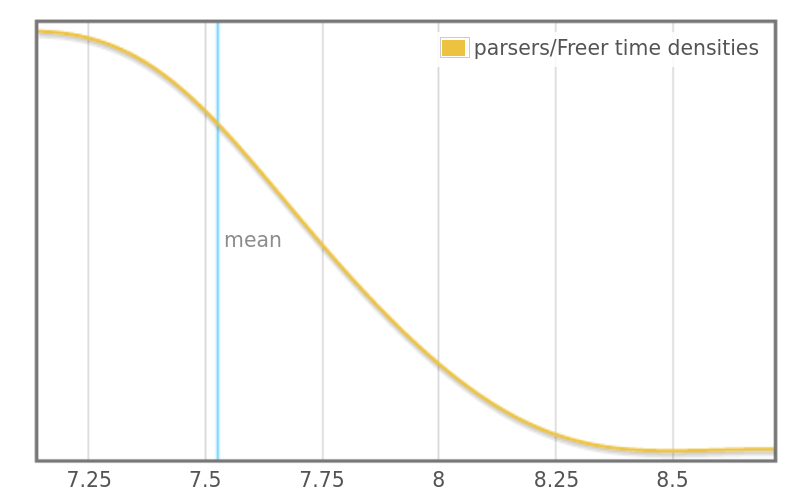
\includegraphics[scale=0.4]{images/freer.png}
      \caption{Monad transformers parsers benchmark}
      \label{mtlParserBench}
      \end{figure}

      The benchmarking was performed for a parser of a Markdown"/like language
      implemented using this library. The benchmarked action was parsing of a
      file of size about 3 kilobytes. The benchmark, together with the source code
      of the library and the parser may be found in the library's GitHub
      repository~\cite{extEffParsers}.

      This benchmark shows extensible effects to work slower in comparison to the monad transformers based implementation (see chapter~\ref{cpt-monads:parsers-bench}).

      \subsection{Conclusion}

      Extensible effects are an embedding of algebraic effects and handlers in Haskell,
      thus the sketched parser combinators library has a lot in common with the one
      implemented in Frank (see previous section). However, as far as Extensible
      Effects are implemented on top of free monads, programmer must adopt the monadic
      style for definition of effectful computations and parsers implementation
      become a bit more wordy than in Frank.
